\begin{footnotesize}
\newcommand{\participK}[2]{
\begin{scope}[shift={(#1)}]
\draw [draw,fill=lightgray] (0pt,10pt) circle (5pt);
\draw [draw,fill=lightgray] (10pt,0pt) arc (0:180:10pt and 5pt);
\fill [lightgray] (-10pt,-10pt) rectangle (10pt,0pt);
\draw [draw] (10pt,0pt) -- (10pt,-10pt);
\draw [draw] (-10pt,0pt) -- (-10pt,-10pt);
\draw [draw] (5pt,-1pt) -- (5pt,-10pt);
\draw [draw] (-5pt,-1pt) -- (-5pt,-10pt);
\draw [anchor=center] (0pt,-2.5pt) node {#2};
\end{scope}
}
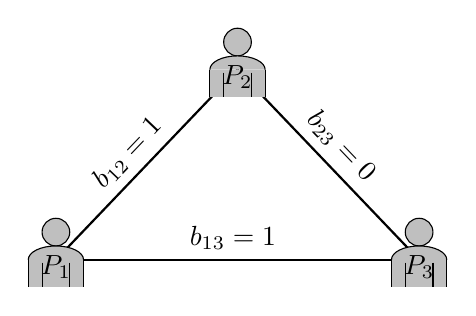
\begin{tikzpicture}
\begin{scope}
\path (18:6.9em) coordinate (P3);
\path (90:9em) coordinate (P2);
\path (162:6.9em) coordinate (P1);
\draw [thick] (P3) to node [anchor=south ,pos=0.5,swap,sloped] {$b_{23} = 0\ $} (P2);
\draw [thick] (P3) to node [anchor=south ,pos=0.5,swap,sloped] {$b_{13} = 1\ $} (P1);
\draw [thick] (P2) to node [anchor=south ,pos=0.5,swap,sloped] {$b_{12} = 1\ $} (P1);

\participK{P1}{$P_1$};
\participK{P2}{$P_2$};
\participK{P3}{$P_3$};
\end{scope}


\end{tikzpicture}
\end{footnotesize}